\documentclass{tufte-handout}

\title{Correlation and Regression}

%\author[The Tufte-LaTeX Developers]{The Tufte-\LaTeX\ Developers}

\date{} % without \date command, current date is supplied

%\geometry{showframe} % display margins for debugging page layout

\usepackage{graphicx} % allow embedded images
  \setkeys{Gin}{width=\linewidth,totalheight=\textheight,keepaspectratio}
  \graphicspath{{graphics/}} % set of paths to search for images
\usepackage{amsmath}  % extended mathematics
\usepackage{booktabs} % book-quality tables
\usepackage{units}    % non-stacked fractions and better unit spacing
\usepackage{multicol} % multiple column layout facilities
\usepackage{lipsum}   % filler text
\usepackage{fancyvrb} % extended verbatim environments
  \fvset{fontsize=\normalsize}% default font size for fancy-verbatim environments

\usepackage{pgfplots}
\pgfplotsset{compat=1.12}

% Standardize command font styles and environments
\newcommand{\doccmd}[1]{\texttt{\textbackslash#1}}% command name -- adds backslash automatically
\newcommand{\docopt}[1]{\ensuremath{\langle}\textrm{\textit{#1}}\ensuremath{\rangle}}% optional command argument
\newcommand{\docarg}[1]{\textrm{\textit{#1}}}% (required) command argument
\newcommand{\docenv}[1]{\textsf{#1}}% environment name
\newcommand{\docpkg}[1]{\texttt{#1}}% package name
\newcommand{\doccls}[1]{\texttt{#1}}% document class name
\newcommand{\docclsopt}[1]{\texttt{#1}}% document class option name
\newenvironment{docspec}{\begin{quote}\noindent}{\end{quote}}% command specification environment

\begin{document}

\maketitle% this prints the handout title, author, and date

\begin{marginfigure}[10pt]
  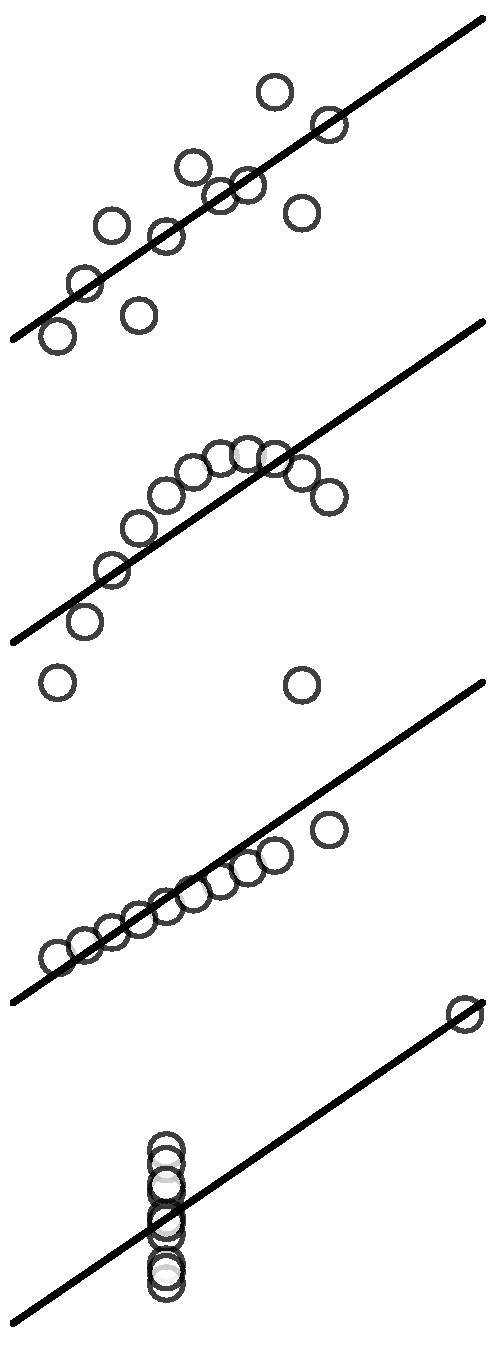
\includegraphics[width=\linewidth]{handout8_anscombe}%
  \label{fig:fullfig}%
  \setfloatalignment{t}
\caption{Anscombe's Quartet. Four datasets with the same $\bar{X}$, $\bar{Y}$,$s_X$,$s_Y$, and correlation coefficient. We often assume that our data is distributed similarly to the top figure, but non-linear trends, and outliers can dramatically affect the interpretation of data.}
\end{marginfigure}


\begin{marginfigure}[20pt]
  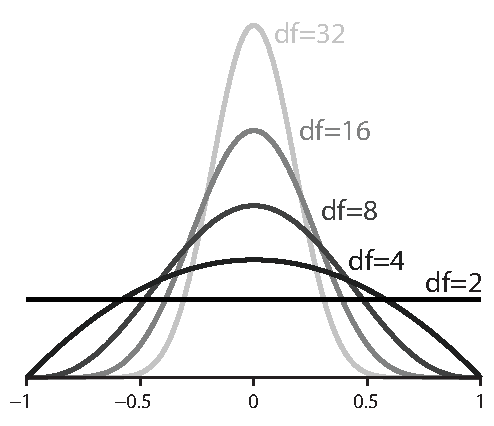
\includegraphics[width=\linewidth]{handout8_rpdf}%
  \label{fig:fullfig}%
  \setfloatalignment{t}
\caption{Null distributions for Pearson correlation with different degrees of freedom $df$.}
\end{marginfigure}

\section{Pearson Correlation}

In summarizing the relationship between two variables, the most common statistic is Pearson's correlation coefficient $r$. As we've discussed, associations can be qualitatively summarized by their \emph{direction} (positive vs negative), \emph{form} (linear vs nonlinear), and \emph{strength} (strong vs weak). The Pearson correlation varies between -1 and 1 and naturally captures the direction and strength of a linear association.

The Pearson correlation is estimated by

\begin{equation*}
r = \frac{\sum (X-\bar{X})(Y-\bar{Y})}{\sqrt{\sum (X-\bar{X})^2 \sum (Y-\bar{Y})^2}}
\end{equation*}

Breaking down the equation we can separate it into two components - the numerator estimates the covariability, the extent to which $X$ and $Y$ tend to vary together

\begin{equation*}
SP=\sum (X-\bar{X})(Y-\bar{Y})
\end{equation*}

The demoniator, uses the sums of squares for $X$ and $Y$, respectively

\begin{equation*}
SS_X=\sum (X-\bar{X})^2 \qquad SS_Y=\sum (Y-\bar{Y})^2
\end{equation*}

Based on this breakdown, we see that the correlation coefficient is a ratio comparing the covarability to the individual variabilities of $X$ and $Y$...

\begin{equation*}
r=\frac{SP}{\sqrt{SS_X SS_Y}}
\end{equation*}

As with the other hypothesis tests, a common step after computing the test statistic is to ask whether or not the association is statistically significant. That is, we want to test the null hypothesis that the population correlation $\rho=0$. Describing the null distribution exactly is a bit outside the scope of this course, but keep in mind that, as with the t-tests and ANOVA, it's shape depends on a degrees of freedom $df=n-2$.

\section{Spearman Correlation}
When the relationship between $X$ and $Y$ is nonlinear or when there are outliers (e.g. the last figure in Anscombe's quartet), Pearson correlation doesn't provide an accurate description of the association. For these trends, a common alternative to the Pearson correlation is the Spearman rank correlation. To compute Spearmann correlation we first convert the $X$ and $Y$ scores to \emph{ranks} (corresponding to the order in a sorted list). The dataset $X:{5,2,10,3}$ for instance, would have ranks $x:{3,1,4,2}$. Identical scores are assigned an average rank, e.g. $X:{1,2,2}\to x:{1,2.5,2.5}$. Once we have the ranks, then find differences between ranks in $X$ and $Y$, $d_i=x_i-y_i$ and we can calculate

\begin{equation*}
\rho=1-\frac{6\sum d_i^2}{n(n^2-1)}
\end{equation*}

Note that if the $X$ ranks and $Y$ ranks are exactly the same, then $d_i=0$ for all $i$ and $\rho=1$. In general there will be some differences between the ranks, but, as with the Pearson corrleation, the Spearman correlation is between -1 and 1 with larger absolute values denoting stronger associations and the same distinction between positive and negative associations.

\section{Linear Regression}

Although, correlation does not imply causation, an important feature of correlations is that they allow one variable to be predicted from the other. With only $X$ and $Y$ we can make this prediction concrete by finding a "line of best fit." This will allows us to take a new value of $X$ and predict what the score for $Y$ should be. Recall that a linear equation in one variable can take the form $\dots$

\begin{equation*}
\hat{Y}=mX+b
\end{equation*}

where $m$ is the slope of the line and $b$ defines the y-intercept. It turns out that after calculating the Pearson correlation coefficient the line of best fit is given by

\begin{equation*}
m=r\frac{s_x}{s_y} \qquad b=\bar{Y}-m\bar{X}
\end{equation*}


\begin{marginfigure}[10pt]
  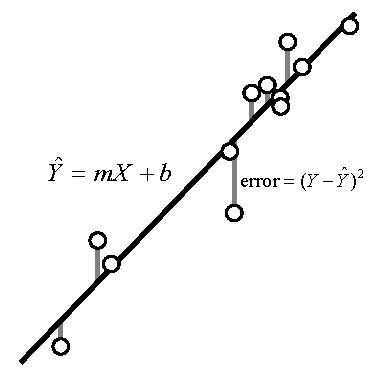
\includegraphics[width=\linewidth]{handout8_bestfit}%
  \label{fig:fullfig}%
  \setfloatalignment{t}
\caption{Line of Best Fit. The line of best fit minimizes errors between observed $Y$ and predicted $\hat{Y}$}
\end{marginfigure}


We write $\hat{Y}$ (pronounced "y-hat") rather than just $Y$ to denote the fact that this equation is an estimate for the value of $Y$. When $-1<r<1$ there will certainly be some errors. The reason that this these equations are the "best fit" is that these errors are minimized.

Regression is a powerful tool in psychology and many other fields. We will not spend much time on it here, but if you continue in statistics you will learn about models with multiple dimensions (e.g. estimating SAT scores based on high-school GPA, socio-economic status, other predictors) and how to model nonlinear relationships between variables.

\pagebreak
\section{Example}

     5     0
    -4     1
     3     2
    -2     7
    13    -2
     0     2
     7     1
     2     5

\pagebreak
\section{Solution}

     5     0     2    -2    -4
    -4     1    -7    -1     7
     3     2     0     0     0
    -2     7    -5     5   -25
    13    -2    10    -4   -40
     0     2    -3     0     0
     7     1     4    -1    -4
     2     5    -1     3    -3
mean   3     2
ss  204    56
sp = -69

r = -0.6456
p = -0.3382    3.0147
sd   5.3984    2.8284
\end{document}

